\input{settings}
\setlength{\emergencystretch}{2em}
\titleformat{\section}
  {\small\bfseries\raggedright}
  {}{0em}
  {}
  [{\color{WHU_Blue}\titlerule}]
\titlespacing*{\section}{0cm}{0.70em}{0.45em}
\titlespacing*{\subsection}{0cm}{0.50em}{0.30em}
\setlist[itemize]{topsep=0.10em, itemsep=0.10em, parsep=0em, partopsep=0em, leftmargin=1.25em}
\setlist[enumerate]{topsep=0.10em, itemsep=0.10em, parsep=0em, partopsep=0em, leftmargin=1.35em}
\renewcommand{\arraystretch}{0.98}
\renewcommand{\CJKglue}{\hskip 0.018em}

% 个人信息
%  cd C:\Users\31087\Documents\Obsidian_Vault\Resume\template
%  xelatex main_scconsult.tex
\newcommand{\school}{江南大学 · 控制科学与工程}

\newcommand{\contact}{
    \scriptsize
    \textcolor{white}{
        \faEnvelope \quad \href{mailto:yuejinai55@gmail.com}{yuejinai55@gmail.com}
        \hspace{3em}
        \faPhone \quad +86 15515602693
        \hspace{3em}
        \faGithub \quad \href{https://github.com/L-yb555}{github.com/L-yb555}
    }
}

\newcommand{\resumeDecor}{
    \begin{tikzpicture}[remember picture, overlay]
        \node[anchor=north, inner sep=0pt](header) at (current page.north){
            
\includegraphics[width=\paperwidth]{images/header.png}
        };
        \node[anchor=west](school_logo) at (header.west){
            \hspace{0.5cm}
            
\includegraphics[width=0.15\textwidth]{images/whu_logo_1.png}
        };
        \node[anchor=east](school_name) at(header.east){
            \textcolor{white}{\textbf{\school}}
            \hspace{0.5cm}
        };
    \end{tikzpicture}

    \begin{tikzpicture}[remember picture, overlay]
        \node[anchor=south, inner sep=0pt](footer) at (current page.south){
            
\includegraphics[width=\paperwidth]{images/footer.png}
        };
        \node[anchor=center] at(footer.center){\contact};
    \end{tikzpicture}

    \begin{tikzpicture}[remember picture, overlay]
        \node[opacity=0.05] at(current page.center){
            
\includegraphics[width=0.68\paperwidth, keepaspectratio]{images/whu_logo_big.png}
        };
    \end{tikzpicture}
}

\newcommand{\sectionIcon}[2]{\makebox[\widthof{#1}][c]{\color{WHU_Blue}{#1}}\quad #2}

%%%%%%%%%%%%%%%%%%%%
% 简历正文
%%%%%%%%%%%%%%%%%%%%
\begin{document}
\resumeDecor
\vspace*{-3.15em}
\scriptsize
\linespread{1.11}\selectfont

% 个人信息
\begin{minipage}{0.80\textwidth}
    \section[个人信息]{\sectionIcon{\faAddressCard}{个人信息}}
    \begin{tabularx}{\linewidth}{p{\widthof{求职意向:}}Xp{\widthof{最高学历:}}X}
        姓\ \ \ \ \ \ \ \ 名: & 梁邦一 &
        性\ \ \ \ \ \ \ \ 别: & 男 \\
        年\ \ \ \ \ \ \ \ 龄: & 24岁 &
        政治面貌: & 共产党员 \\
        英语等级: & CET-6 &
        求职意向: & Associate Consultant \\
    \end{tabularx}
\end{minipage}
\hfill
\begin{minipage}{0.12\textwidth}
    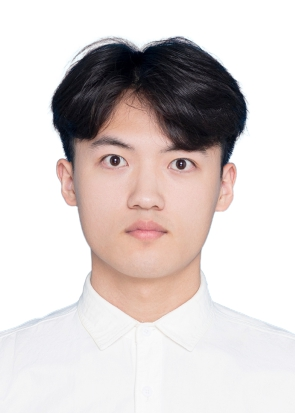
\includegraphics[width=\linewidth]{images/avatar.png}
\end{minipage}
\vspace{-1.28em}

\section[教育背景]{\sectionIcon{\faGraduationCap}{教育背景}}
\begin{itemize}
    \item {\textbf{控制科学与工程硕士，江南大学}} \hfill {2024.06--2027.06}
    \item {\textbf{自动化学士，郑州轻工业大学}}（PLC 编程、传感器与检测、微机原理、嵌入式系统） \hfill {2020.09--2024.06}
\end{itemize}

% 荣誉与组织经历
\section[荣誉与组织经历]{\sectionIcon{\faStar}{荣誉与组织经历}}
\begin{itemize}
    \item \textbf{中国机器人大赛暨 RoboCup 机器人世界杯中国赛} 国家三等奖（本科期间）；校一等奖学金（2025.10）；优秀毕业生（2024.06）。本科班长（4 年，60 人班级）、硕士党支部书记，6 年学生干部经历。
\end{itemize}

% 专业技能
\section[专业技能]{\sectionIcon{\faWrench}{专业技能}}
\begin{itemize}
    \item \textbf{工业 AI 算法与多源数据处理}：Python、C++、\textbf{PyTorch、OpenCV、Pandas}、Ultralytics YOLO；熟悉 CNN、\textbf{Transformer、Conformer、Grounding DINO、Qwen3-VL} 等；具备\textbf{分类、检测、分割、连续值回归、时序建模、异常检测}训练/验证/bad case 归因经验；熟悉 \textbf{Prompt Engineering、LoRA / SFT、GRPO}；掌握多源数据清洗、降噪、特征提取、标签构建、Corner Case 合成等数据侧完整流程。
    \item \textbf{算法部署与工程落地}：Linux/Ubuntu、Git、bash；4 机 8 卡 H20 集群多机多卡分布式训练；R11 人形机器人视觉模型端侧部署与推理性能验证实践；\textbf{边缘部署与工业协议方向储备}（TensorRT / ONNX / Docker / Kubernetes、Modbus / OPC UA、SCADA / MES）。
    \item \textbf{工业场景理解与跨团队协作}：自动化本科背景，熟悉 \textbf{PLC 编程}、控制逻辑设计、设备规格解读；本科在汽车制造一线完成 PLC 控制程序优化并交付生产验证；对接算法、标注、验收多方需求；6 年学生干部沉淀跨角色沟通与需求转技术方案能力。
\end{itemize}

% 实习经历
\section[实习经历]{\sectionIcon{\faBriefcase}{实习经历}}

\vspace{0.04em}
{\normalsize\textbf{CARIZON（大众×地平线合资智驾）}}  感知数据部门算法实习生 \hfill {2026.06--至今}\\
\textbf{AI 场景技术路径设计 / 多源异构数据处理 / 深度学习+机器学习+时序算法组合开发}
\begin{enumerate}
    \item \textbf{AI 场景技术路径与方案输出}：面向感知数据业务需求（长尾场景、Corner Case、细粒度识别），设计"\textbf{规则 Tagger（机器学习）+ 开放词汇检测（Grounding DINO）+ VLM 后训练（大模型）}"分层技术路径，输出可迭代算法解决方案 — 可迁移到\textbf{制造业缺陷识别、工艺优化、仓储策略}等场景。
    \item \textbf{多源异构数据处理与算法开发}：处理车载多路结构化数据 + 回灌数据 + 图像数据，完成数据清洗、时间戳对齐、Prompt 迭代、Corner Case 数据合成、标签构建；在 3W 条路口数据中筛选 3K 条转向 CLIP（\textbf{标签验收准确率达 90\%}）；设计"规则渲染 + 生成模型"合成 pipeline 产出 5K 张 Corner Case 样本，覆盖分类、检测、细粒度识别多任务算法开发。
    \item \textbf{大模型后训练与业务交付}（可类比制造业缺陷识别）：负责泊车障碍物 VLM 优化，筛选 1.8 万张挡轮杆图像完成清洗、标注校验与 Prompt 迭代；基于 \textbf{Qwen3-VL-8B + LLaMA-Factory} 在 \textbf{4 机 8 卡 H20 集群完成全参数 SFT}；针对验收问题设计\textbf{基于 GRPO 的三元组策略优化方法}，完成模型二次精标业务交付。
\end{enumerate}

\vspace{0.04em}
{\normalsize\textbf{优奇智能科技有限公司（优必选子公司）}}  人形机器人感知算法实习生 \hfill {2026.02--2026.05} \\
\textbf{机器人端视觉模型部署 / 推理性能验证 / 边缘设备工程环境}
\begin{enumerate}
    \item \textbf{视觉模型部署与推理性能验证}：参与 R11 接待机器人感知模块 \textbf{YOLO11s-seg} 模型训练与\textbf{机器人端部署验证}，在 Ubuntu 环境完成实验环境搭建、数据配置、训练参数调整与效果验证；关注模型在\textbf{边缘设备（机器人端）}的推理性能与部署效率，具备将检测/分割模型迁移到端侧的实践基础。
    \item 负责多场景视觉数据清洗、类别一致性检查、标注质检及训练/验证/测试集划分；围绕误检、漏检与分割边界不稳定 bad case 归因，建立"模型评估 → 问题归因 → 数据改进"迭代闭环；具备 \textbf{TensorRT / ONNX / Docker} 等边缘部署方向储备。
\end{enumerate}

\vspace{0.04em}
{\normalsize\textbf{长兴和良智能制造有限公司}}  研发实习生 \hfill {2024.05--2024.09} \\
\textbf{制造业一线 / PLC 控制程序优化 / 需求转技术方案}
\begin{enumerate}
    \item 深度参与汽车制造流程，负责核心生产设备（汽车空调弯管机）\textbf{PLC 控制程序优化项目}，将业务需求转化为可执行技术方案；独立完成设备规格书解读、流程文档设计与生产验证，方案在实际生产环境稳定运行，积累\textbf{"现场需求 → 控制逻辑 → 交付验证"}完整工程经验，形成对工业自动化设备与 PLC 编程的一手认知。
\end{enumerate}

\vspace{0.04em}
{\normalsize\textbf{机器人与智能系统全国重点实验室（中国科学院沈阳自动化研究所）}}  实习生 \hfill {2025.02--2026.02} \\
\textbf{前沿技术调研 / 综述论文写作 / 多模态实验平台}
\begin{enumerate}
    \item \textbf{前沿技术探索}：\textbf{系统性梳理}感知、人机交互与机器人方向英文文献，归纳传感器方案、算法框架、数据集与应用场景，支撑综述论文写作与技术路线判断（成果见下方 IEEE Sensors Journal 综述） — 可迁移到\textbf{工业 AI 前沿技术调研与创新场景试点评估}；同时独立完成 Linux 服务器环境搭建与维护，保障 PyTorch 训练与实验复现稳定运行。
\end{enumerate}

\vspace{0.04em}
\section[科研与项目经历]{\sectionIcon{\faFlask}{科研与项目经历}}

\vspace{0.04em}
{\normalsize\textbf{面向具身智能灵巧操作的多模态感知与控制系统（灵心巧手） · 负责人}} \hfill {2025.02--2026.02} \\
\textbf{ 端到端项目负责人 / 时序建模 / 模块化系统方案 \hfill GitHub: \href{https://github.com/L-yb555/semg-force_ui}{github.com/L-yb555/semg-force\_ui}}
\begin{enumerate}
    \item \textbf{独立牵头}多模态感知系统从 0 到 1 建设，拆解为硬件采集 → 算法训练 → 仿真验证 → ROS2 联调 → Web/VR 演示 5 大阶段，历时 12 个月完成端到端项目闭环；基于 PyTorch 开展 \textbf{Transformer / 轻量 Conformer 时序建模}，多通道 sEMG 信号支持力等级分类 + 连续力值回归双任务；设计模块化 ROS2 Topic 接口 — 可迁移到\textbf{工业时序异常检测、设备状态识别与预测性维护}。
\end{enumerate}

\section[论文与研究成果]{\sectionIcon{\faBook}{论文与研究成果}}
\begin{enumerate}
    \item 已中（JCR 一区，中科院二区）：Liang B., Li N., Li G., et al. Sensing Technologies for Hand Gesture Recognition in Human-Robot Interaction: A Review[J]. IEEE Sensors Journal, 2025, 26(2): 1501-1519.
    \item 在修（JCR 一区，中科院二区 Top）：sEMG Conformer: Synergizing Local-Global Spatiotemporal Features for Continuous Force Estimation. Biomedical Signal Processing and Control.
    \item 在投（JCR 一区，中科院二区）：Dexterous Hand Grasping Control Based on Multimodal Sensory Fusion and Simulation Reinforcement Learning.
\end{enumerate}

\end{document}
